\documentclass{article}
\usepackage{relsize}
\usepackage{tikz} % ,pgf,pgfarrows,pgfnodes,pgfautomata,pgfheaps,pgfshade}
\usetikzlibrary{shapes,decorations,shadings,positioning,arrows}
\tikzstyle{legend} = [red, fill=white, font=\footnotesize, inner sep=2pt, rounded corners=0.05cm]
\tikzstyle{arrow} = [red, ->, line width=2pt]

\usepackage{amsmath,enumerate,xspace,subfig,siunitx,lscape}
\usepackage{listings}
\usepackage[absolute,overlay]{textpos}

\usepackage[colorlinks=true,linkcolor=red,pagecolor=red,
  citecolor=blue,urlcolor=blue,breaklinks=true,
  hyperfootnotes=false,pdftitle={CombLayer Guide},
  pdfauthor={Stuart Ansell},pdfkeywords={CombLayer,MCNP,MCNPX}]
           {hyperref}
\renewcommand*{\rmdefault}{cmss} 


\definecolor{SlateBlue}{rgb}{0.1,0.1,1.00}
\definecolor{SlateGreen}{rgb}{0.1,0.8,0.3}
\definecolor{darkred}{rgb}{0.8,0,0}
\newcommand{\tcg}[1]{
   \textcolor{green}{#1}}
\newcommand{\tcr}[1]{
   \textcolor{red}{#1}}
\newcommand{\tcb}[1]{
   \textcolor{blue}{#1}}
\newcommand{\tcbb}[1]{
   \textcolor{SlateBlue}{#1}}
\newcommand{\tcgg}[1]{
   \textcolor{SlateGreen}{#1}}


\definecolor{mygray}{rgb}{0.4,0.4,0.4}
\definecolor{mygreen}{rgb}{0,0.8,0.6}
\definecolor{myorange}{rgb}{1.0,0.4,0}

\lstset{
  basicstyle=\small\sffamily\color{black},
  commentstyle=\color{red},
  frame=false,
  numbers=left,
  numbersep=5pt,
  numberstyle=\tiny\color{mygray},
  keywordstyle=\color{blue},
  showspaces=false,
  showstringspaces=false,
  stringstyle=\color{myorange},
  tabsize=8,
  otherkeywords={std},
  escapeinside={\%\%}{\@},
  xleftmargin=0.0\linewidth
}
\newcommand {\prog}[1]{{\it #1}}
\newcommand {\vb}[1]{\begin{\verbatim}{#1}\end{verbatim}}
\newcommand {\alert}[1]{\textcolor{red}{#1}}
\lstnewenvironment{bash}{\lstset{language=bash,numbers=none,backgroundcolor=\color{yellow!20},frame=tb}}{}
\lstnewenvironment{cpp}{\lstset{language=C++,numbers=none,backgroundcolor=\color{green!10},frame=tb}}{}
\lstnewenvironment{deck}{\lstset{language=bash,numbers=none,backgroundcolor=\color{gray!10},frame=tb}}{}
\lstnewenvironment{xml}{\lstset{language=xml,numbers=none,backgroundcolor=\color{green!10},frame=tb}}{}

\setlength{\parindent}{0in}
\setlength{\parskip}{0.1in}
\setlength{\textwidth}{6.5in}
\setlength{\textheight}{9.0in}
\setlength{\oddsidemargin}{0.0in} 
\setlength{\evensidemargin}{0.0in} 

\newcommand{\mcnp}{{\tt MCNP}\xspace}
\newcommand{\cinder}{{\tt CINDER}\xspace}

\newcommand{\figref}[1]{Fig.\,\ref{#1}}
\newcommand{\figrefp}[1]{Fig.\,\ref{#1} on page~\pageref{#1}}

\newcommand{\secref}[1]{Sec.\,\ref{#1}}
\newcommand{\secrefp}[1]{Sec.\,\ref{#1} on page~\pageref{#1}}


\newcommand{\drawMug}[3]{
  \def\width{4};
  \def\height{5};
  \coordinate (A) at (#1,#2);
  \coordinate (B) at (#1+\width,#2+\height);
  \draw[#3] (A) rectangle (B);
  \draw[#3] (#1,3) arc (90:270:1cm);
  \draw[#3] (#1,3.3) arc (80:280:1.3cm);
}

\newcommand{\drawSpoon}[3]{
  \def\hWidth{0.5};
  \def\hHeight{5};
  \def\lWidth{0.3};
  \def\lHeight{1.5};
  % ladle
  \coordinate (C) at (#1-\lWidth,#2);
  \coordinate (D) at (#1+\hWidth+\lWidth,#2+\lHeight);
  \draw[#3] (C) rectangle (D);
  % handle
  \coordinate (A) at (#1,#2+\lHeight);
  \coordinate (B) at (#1+\hWidth,#2+\hHeight);
  \draw[#3] (A) rectangle (B);
}


\title{CombLayer Guide}
\author{Stuart Ansell}

\begin{document}
\maketitle
\tableofcontents

\input{Frames/Introduction}
\newpage
\input{Frames/Layout}
\input{Frames/Installing}
\input{Frames/LinkSystem}
\input{Frames/ModelInitial}
\input{Frames/TallySystem}
%\section{HowTo}
\begin{itemize}
\item Get real surface number by its relative number: SMap.realSurf(divIndex+103) (see createLinks methods)
\end{itemize}

\subsection{How to put one object into another}

Suppose, we are inserting Spoon into Mug.
Mug is made up of N cells. Spoon is made of one contained component with outer surface.
CombLayer provides several methods to put one object into another:

\begin{cpp}{Name=essBuild}{floatplacement=H}
attachSystem::addToInsertForced(System,   *Mug, *Spoon);
attachSystem::addToInsertSurfCtrl(System, *Mug, *Spoon);
attachSystem::addToInsertControl(System,  *Mug, *Spoon);
attachSystem::addToInsertLineCtrl(System, *Mug, *Spoon);
\end{cpp}

\subsubsection{addToInsertForced}

The outer surface of the Spoon is excluded from the HeadRule of every single cell of Mug.
Even if Mug contains cells which do not intersect with Spoon (e.g. its handle, see \figref{fig:forced}).
{\it Forced} means {\it do it and do not think about it}, but at the same time it means that
{\it I have got something wrong somewhere.}  Normally this is that insufficient link points have been added
to the object, or that the object is a set of split (single cell) volumes.  However, there is the additional
problem that the model may not be correctly constructed at this point, so that the other options seem not to work.
This can be checked by adding a
\prog{SimProcess::writeIndexSim(System,"OutputFilename.txt",0);}
in the code just before the call to insertForced. If there are undefined volumes then the model is not in a state that
any of the \prog{addToInsert} algorithms except \prog{addToInsertForced} can be used. 

\begin{figure}
  \centering
  \begin{tikzpicture}
    \drawMug{0}{0}{}
    \drawSpoon{2}{1}{dashed}
  \end{tikzpicture}
  \caption{addToInsertForced: all cells of Spoon are excluded from all cells of Mug including non intersecting cells}
  \label{fig:forced}
\end{figure}


\subsubsection{addToInsertSurfCtrl}

The objective of this function is to use the surface intersections between Mug and spoon to determine which 
cells within Mug intersect the ContainedComp of spoon. The process is done on a cell - ContainedComp level. 

The process is as follows:
\begin{enumerate}

\item{Deconvolves both the Spoon's containedComponent boundary into surfaces.}
\item{Loop over each cell in Mug : MCell}
  \begin{enumerate}
  \item{Calculate intersection of each surface:surface:surface triplet from the set of CC surfaces and MCell surface}
  \item{If a point is within CC and the MCell exclude the CC from the
    MCell and goto next cell}
  \end{enumerate}
\end{enumerate}
   
Thus the spoon is inserted only into those cells of Mug which it intersects~(\figref{fig:surfctrl}).

It is not always better to call {\tt addToInsertSurfCtrl} instead of
{\tt addToInsertForced} in cases that if is certain that an
intersection can must take place (particularly if the CC / Inserting
cells have large numbers of surfaces).

{\tt addToInsertSurfCtrl} is a very expensive function to call,
because you have to check all the surface triplets. So, it runs a bit
slower than addToInsertForced, but the geometry will be faster.

\begin{figure}
  \centering
  \subfloat[Cell 3 is excluded from cell 1; cells 2 and 4 not changed]{
    \begin{tikzpicture}
      \drawMug{0}{0}{}
      \drawSpoon{2}{4}{dashed}
      \node[legend] at (2,2) {1};
      \node[legend] at (-1.25,2) {2};

      \node[legend,blue,fill=white] at (2.25,4.5) {3};
      \node[legend,blue,fill=white] at (2.25,6) {4};
    \end{tikzpicture}
  } \quad
  \subfloat[None of the cells are modified]{
    \begin{tikzpicture}
      \drawMug{0}{0}{}
      \drawSpoon{5}{1}{dashed}
      \node[legend] at (2,2) {1};
      \node[legend] at (-1.25,2) {2};

      \node[legend,blue,fill=white] at (5.25,2) {3};
      \node[legend,blue,fill=white] at (5.25,3) {4};
    \end{tikzpicture}
  }
  \caption{addToInsertSurfCtrl: only needed cells are excluded}
  \label{fig:surfctrl}
\end{figure}

The two remaining methods provide similar functionality but with less
computational overhead, however, there are cell constructs which will
cause them to fail.


\subsubsection{addToInsertControl}

It's a very simple method. The link points from Spoon are uses as a test for each of the cells within Mug. 
The method checks if any of these link point fit inside each of the cells of Mug. If it does, then it cuts Spoon from the Mug cell~(\figref{fig:control}).
It is possible to add a vector of link points to check as a parameter to limit the search.

\begin{figure}
  \centering
  \subfloat[Cell 3 is excluded from cell 1 since Mug has a link point which is located inside cell 3. Cells 2 and 4 are not modifed. \alert{Compare: The Spoon cells (3 and 4) are excluded from the Mug cells (1 and 2) since Mug has a link point which is located inside a Spoon cell}]{
    \begin{tikzpicture}
      \drawMug{0}{0}{}
      \node[legend] at (2,2) {1};
      \node[legend] at (-1.25,2) {2};
      \draw[red] (2,5) circle (2pt);

      \drawSpoon{2}{4}{dashed}
      \node[legend,blue,fill=white] at (2.25,4.5) {3};
      \node[legend,blue,fill=white] at (2.25,6) {4};
      \draw[blue] (2.25,4) circle (2pt);
    \end{tikzpicture}
  } \quad
  \subfloat[Intersection is not made since none of link points are located in another component. Geometry is broken. To fix it, define more link points or use another volume inclusion method. \alert{check}]{
    \begin{tikzpicture}
      \drawMug{0}{0}{}
      \node[legend] at (2,2) {1};
      \node[legend] at (-1.25,2) {2};
      \draw[red] (-1.53,2) circle (2pt);
      \draw[red] (-1,2) circle (2pt);
      \draw[red] (0,2.5) circle (2pt);

      \drawSpoon{-0.85}{-1}{dashed}
      \node[legend,blue,fill=white] at (-0.6,-0.3) {3};
      \node[legend,blue,fill=white] at (-0.6,3.5) {4};
      \draw[blue] (-0.6,4) circle (2pt);
      \draw[blue] (-0.6,0.5) circle (2pt);
    \end{tikzpicture}
  }
  \caption{addToInsertControl: intersection relies on the link points}
  \label{fig:control}
\end{figure}

\subsubsection{addToInsertLineCtrl}

Imagine we have a (big) contained component~(Mug) and some (small)
object which clips it~(Spoon). The link points are {\bf not} in the
Mug~(therefore {\bf addToInsertControl} can not be used), but the
lines which connect them are in the Mug.  The method checks the lines
connecting the link points and sorts out the intersections.


\section{Components}

\input{Components/ObjectRegister}
\input{Components/ExtWeightCommand}

\section{User guide}
This section describes how to use CombLayer from a user's (i.e. non-developer) point of view.
In this guide, it is assumed that the user has no C++ or coding experience.

The guide is focused on the ESS model, which can be generated by running. 
\begin{bash}
  ./ess -r modelOut
\end{bash}
This command produces the \mcnp input file {\tt modelOut1.x} as well as two other files: {\tt ObjectRegister.txt} and {\tt Renumber.txt}.

The single flag {\tt -r} is optional for MCNP6 as it causes the objects and surfaces in MCNP to be renumbered sequentially and
to fit within the 100,000 object/surface limits of MCNPX.

\subsection{Variables}
In the beginning of the input file there is a commented list of variables which define the geometry:

\begin{deck}
 c ----------------------------------------------
 c --------------- VARIABLE CARDS ---------------
 c ----------------------------------------------
 c ABunkerFloorDepth 120
 c ABunkerFloorThick 100
 c ABunkerLeftAngle 0
 c ABunkerLeftPhase -65
 c ABunkerNLayers 1
 ...
\end{deck}

The variable name consists of the component name and its corresponding parameter. For instance,
the first variable {\tt ABunkerFloorDepth} in the list above sets the floor depth of the component called {\tt ABunker}.

Only variables that have needed to be examined are included in this output. Several components are optional and if not built then
their corresponding variables are not seen in the output. All variables start with an initial value and stateless variables are prohibited.
Most variables are defined appropiately within the CombLayer program and obviously can be changed by editing the code and recompiling.
However for a simple variable change that is excessive work so there are a number of methods to change variables from the command line.

\subsubsection{How to change variables}
Any of these variables can be changed either via a command line arguments or an XML file.

As an example, consider changing the Beryllium reflector height.
First of all, we need to find out which variable we need to change and therefore find out the name of the Be reflector
component in CombLayer.

To do this, open the \mcnp geometry and click on any Be reflector cell. Currently, it's cell number 5~(exact number depends on the
CombLayer version you are using).

Now we need to find out which component this cell belongs to.  Find this cell number in the {\tt Renumber.txt} file:
\begin{bash}
grep " 5 " Renumber.txt 
Surf Change:1000006 5                                                           
Cell Changed :1000005 5 Object:BeRef (topBe)       
\end{bash}
It shows that the corresponding Be reflector object is called {\tt BeRef}.

Now we need to find out which {\tt BeRef} variable is responsible for its height:
\begin{bash}
grep BeRef a1.x 
c BeRefHeight 74.2
c BeRefLowRefMat Be5H2O
c BeRefLowWallMat Stainless304
c BeRefRadius 34.3
c BeRefTargSepMat Void
c BeRefTopRefMat Be5H2O
c BeRefTopWallMat Stainless304
c BeRefWallThick 3
c BeRefWallThickLow 0
\end{bash}

We can guess from this list that the variable we need is called {\tt BeRefHeight}.

\paragraph[Command line]{Changing variables via command line}
In order to change a variable via command line arguments, run:
\begin{bash}
  ./ess -r -v BeRefHeight 50 modelOut
\end{bash}
Several variables can be changed, e.g.:
\begin{bash}
  ./ess -r -v BeRefHeight 50 -v BeRefRadius 35 modelOut
\end{bash}

Note that it is possible that you miss spell one of the variables, if this is the case then
you will be presented 

\begin{bash}
./ess -r -v BeRefHHH 1 modelOut
Failure to find variable name BeRefHHH                     MainProcess[F]::setRunTimeVariable
Exiting from BeRefHHH not found                            ::main
Exit Stack:                                                ::main
::main                                                     ::main
  MainProcess::InputModifications                          ::main
    MainProcess::setVariables                              ::main
      MainProcess[F]::setRunTimeVariable                   ::main
\end{bash}

Like most CombLayer error messages it is expected that you read them from top to bottom. So the first thing it tells you is
that variable BeRefHHH does not exist in the model. Second that this is a fatal error and finally the calling stack that generated
that error. If you are not debugging the code etc, Then only concern yourself with the error/warning messages above the line {\it Exit Stack:}.


It is also possible to use strings and Vec3D objects as variables.

e.g.

\begin{bash}
  ./ess -r -v BeRefTopRefMat Nickel \
           -v ABunkerQuakePtA0 'Vec3D(1200,191.2,0.0)' modelOut
\end{bash}

will set the Top reflector material to {\it Nickel} and the start of the dilitation joint at 1200,191.2,0 (relative to
target centre. Note that on bash you will need to hard quote (single quote) the Vec3D value or it will
be split into commands.


\paragraph[XML file]{Changing variables with XML file}
Create an XML file with the following content:

\begin{xml}
<?xml version="1.0" encoding="ISO-8859-1" ?>
<metadata_entry>
  <Variables>
  <variable name="BeRefHeight" type="double">50</variable>
  <variable name="BeRefTopRefMat" type="string">Nickel</variable>
  </Variables>
</metadata_entry>
\end{xml}

and generate the modified geometry:
\begin{bash}
  ./ess -r -x model.xml modelOut
\end{bash}

All the variables can be exported in the XML file by running
\begin{bash}
  ./ess -r -X modelOut.xml modelOut
\end{bash}
Note that the -X command will overwrite existing files.

The commands can be done combined simulantiously with both XML and command line and output.
\begin{bash}
  ./ess -r -X modelOut.xml -x model.xml -v BeRefHeight 80.0 modelOut 
\end{bash}

This will first read the model.xml file and change the variables. Second it will
change BeRefHeight to 80, and finally write out the XML file of all variables to the file
modelOut.xml.


\subsection{Variance reduction}
\subsubsection{Cell-based biasing}
\label{sec:vr:cell}

Cell-based weight window can be generated with the following arguments:

\lstinputlisting[language=bash,numbers=none,backgroundcolor=\color{yellow!20},frame=tb]{UserGuide/cell-biasing.sh}

\begin{description}
\item[-defaultConfig Single ODIN -angle objAxis odinAxis 0] These optional arguments build the ODIN beam line
  and rotate geometry around the $z$ axis and then the $y$ axis such that the FixedComp linkPt axis specified
  in the -angle command is made collinear with the $x$ axis.
  In this example it is the ODIN beamline axis which is aligned on the $x$ axis.
  This rotation simplifies the weight window source plane setup for the current example and used here for
  illustration purpose~(see \figref{fig:vr:cell}).
\item[-w] should precede all weight-related arguments.
\item[--weightEnergyType] defines energy grid\footnote{With the {\tt wwg} card you can either use this expression or {\tt --wwgE}.}.
  The following variants of syntax are possible:
  \begin{enumerate}
    \item If use the word {\em energy} then the format is energy followed by default weight for that bin
      (in our example: for energies below \SI{0.1}{\mega\electronvolt} the default weight is \num{0.95};
          for energies between \num{0.1} and \SI{1}{\mega\electronvolt} the default weight is \num{0.85} etc).
    \item If you drop the word {\em energy} then you just set the energy grid without specifying default weights and the default weight is taken as 1.0.
    \item Alternatively you can use pre-defined keywords:
      {\tt basic}, {\tt high}, {\tt mid} and {\tt flat}\footnote{Energy-weight binnings for these keywords are defined in \tt{System/weights/WeightControl.cxx}}.
    \end{enumerate}
\item[--weightSource] This argument defines a point in space. We can define as many as we want (by adding several {\tt weightSource} arguments),
  but only those used with {\tt weightObject} will be used.
  This particular point is shown by a circle in the left side of \figref{fig:vr:cell:labels}.
\item[--weightPlane] This argument defines a plane. Similarly to {\tt weightSource}, we can define as many planes as we want,
  but only those used with {\tt weightObject} will be used.
  This particular plane is shown by a dashed vertical line in the right side of \figref{fig:vr:cell:labels}.
\item[--weightObject] Define objects we would like to make cell-based variance reduction to.
  \begin{description}
  \item[G2BLineTop20] Object name.  It's also possible to specify range of objects within an object or cell name via {\tt CellMap}.
  \item[SS0] Refer to the first simple source term (the point defined via {\bf weightSource} above).
    It implies that the point should be considered as a source (i.e. particles are emitted from it).
  \item[TS1] Refer to the second simple source term (the point defined via {\bf weightSource} above).
    It implies that the point should be considered as a tally region, it is calculated in the same way as
    as source term but the weight contribute is calculated as the reciprical of the contribution (inverted with respect to SS0).
    \item[energyCut=0.0] Energy cut. Defines min energy for variance reduction (i.e. no variance reduction below this energy will be made~--- default weight will be used as defined in weightEnergyType. If energyCut is less than 0.0 then it defines the maximum energy for variance reduction.
    \item[scaleFactor=1.0] Linear scale factor. You are going to work out an exponent which is
      the scattering term into something. It's $ \textrm{scaleFactor} \exp(-\sigma \rho /
           {\textrm r2len} r)^{\textrm{r2Pow}} )$.
      It's transport to go from {\em a} cell to another cell. \alert{Scale factor is taken out in the mesh based variance reduction.}
    \item[density=0.9] Density scale factor. Normally we set it a bit less than one to make it easier to do transport through thick layers.
    \item[r2Len=1.0] Length scale factor \alert{Do not understand}
    \item[r2Pow=2.0] Scale for the length exponent in $r^{\text{r2Pow}}$.
  \end{description}

 % {\tt TP1}: tally plane 1;
 %  \mbox{\tt 1.0 1.0 0.15 1e-20}: energy above \SI{1}{\mega\electronvolt} (below it we are not interested~--- use default values);
 %  {\tt 1.0}: scale factor; 
 %  {\tt 0.15}: density factor; {\tt 1e-20}: minimum weight % 41:12
\item[--voidUnMask] By default the importance of the void cell surrounding geometry is 0. This argument sets it to 1.
  It can be useful if we believe that particles travelling through that cell can contribute into the tally.
  It's always recommended to put this flag unless you really understand what you are doing.
\end{description}

\paragraph{Notes}
\begin{itemize}
\item In order to set up biasing, you need at least one source. If you have one tally you must also have at least one source, If several tallies are used, then the weight is multipied together, however at each stage
  normalization to the source is carried out. Therefore the order is important.
\item Source can be defined either as a point (via {\bf --weightSource}) or a plane (via {\bf --weightPlane}). In the example above we defined point source.
  However the defined sources and planes do nothing until you use them in {\bf --weightObject} or somewhere else.
\item General rule to get the things into work: try different setups and compare results. Then you renormalise it back out again. It's just basically numerical level game.
  Very often SA scales by this and then rescales by that.
\end{itemize}

% \begin{equation}
%   \label{eq:vr:cellweight}
%   W = \exp{(-w \cdot \sigma_{\text{scale}} \cdot \text{scaleFactor} \cdot \text{factor})}
% \end{equation}

% % CellWeight.cxx
% $$
% factor = minW < \num{1e-16} ? log(\num{1e-16})/log(minW) : 1.0
% $$


\begin{landscape}
\begin{figure}
  \centering
  \subfloat[Horizontal view: geometry \label{fig:vr:cell:labels} ]{
  \begin{tikzpicture}
    \node[anchor=south west,inner sep=0] (image) at (0,0) {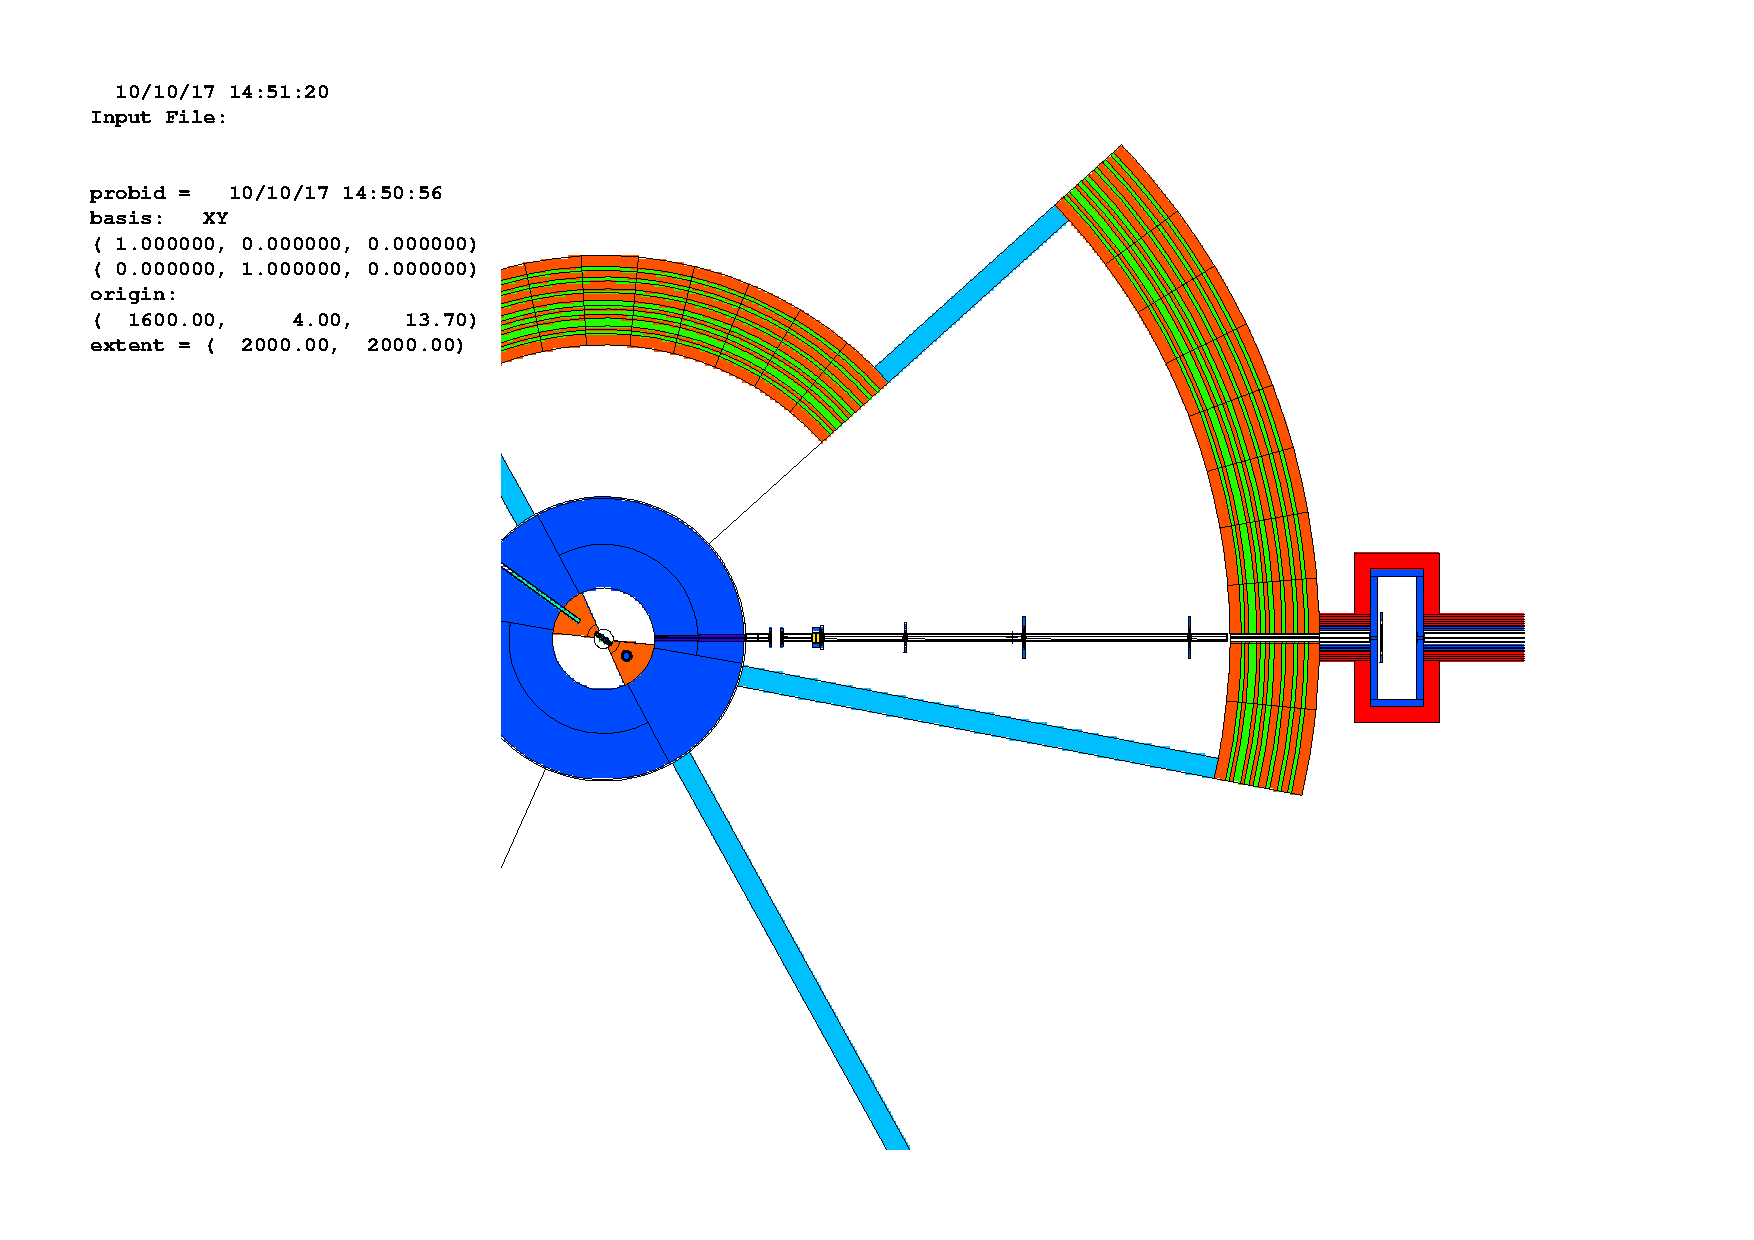
\includegraphics[width=0.5\linewidth,page=1,clip=true, trim=10cm 8cm 4cm 7cm]{UserGuide/cell-biasing.pdf}};
    \begin{scope}[x={(image.south east)},y={(image.north west)}]
      % \draw[help lines, xstep=.1, ystep=.1] (0,0) grid (1,1);
      % \foreach \x in {0,1,...,9} {\node [anchor=north] at (\x/10, 0) {0.\x}; }
      % \foreach \y in {0,1,...,9} {\node [anchor=east]  at (0, \y/10) {0.\y}; }

      \draw[red,thick] (0.07, 0.367) circle (0.5mm);
      \draw[arrow] (0.11,0.46) -- (0.077,0.38);
      \node[legend, anchor=west] at (0.1,0.5) {weightSource};

      \draw[red,dashed] (0.79,0) -- (0.79,1);
      \draw[arrow] (0.85,0.8) -- (0.79,0.8);
      \node[legend, anchor=west] at (0.85,0.8) {weightPlane};

      \draw[arrow]     (0.14,0.2) -- (0.14,0.36);
      \node[legend] at (0.14,0.2) {G2BLineTop20};

      \draw[arrow]                 (0.65,0.25) -- (0.69,0.25);
      \node[legend,anchor=east] at (0.65,0.25) {CBunkerWallMainWall1};

      \draw[arrow]                 (0.65,0.45) -- (0.69,0.45);
      \node[legend,anchor=east] at (0.65,0.45) {CBunkerWallMainWall2};
    \end{scope}
  \end{tikzpicture}
  }
  \subfloat[Horizontal view: wwn]{
    \includegraphics[width=0.5\linewidth,page=2,clip=true, trim=10cm 8cm 4cm 7cm]{UserGuide/cell-biasing.pdf}
  } \\
  \subfloat[Vertical view: geometry]{
    \includegraphics[width=0.5\linewidth,page=3,clip=true, trim=10cm 8cm 4cm 7cm]{UserGuide/cell-biasing.pdf}
  }
  \subfloat[Vertical view: wwn]{
    \includegraphics[width=0.5\linewidth,page=4,clip=true, trim=10cm 8cm 4cm 7cm]{UserGuide/cell-biasing.pdf}
  }
  \caption{Cell-based weight window}
  \label{fig:vr:cell}
\end{figure}
\end{landscape}


\end{document}


\end{document}
